%----------------------------------------------------------------------------------------
% PACKAGES AND OTHER DOCUMENT CONFIGURATIONS
%----------------------------------------------------------------------------------------

\documentclass[9pt]{./src/packages/Developer_CV/developercv}
\usepackage{amssymb}
\usepackage{fontawesome}
\usepackage{enumitem}
\usepackage{ifpdf}
\graphicspath{ {./img/} }

\begin{document}

%----------------------------------------------------------------------------------------
% PHOTO, NAME, CONTACT
%----------------------------------------------------------------------------------------

\begin{minipage}[t]{0.15\textwidth} % 30% of the page width for photo
    \vspace{-\baselineskip} % Required for vertically aligning minipages
    \raggedright % Align to left as possible
    \setlength{\fboxsep}{0pt} % Removes the gap between the image and the border
    \setlength{\fboxrule}{3pt} % Add border
    \ifpdf
        \fbox{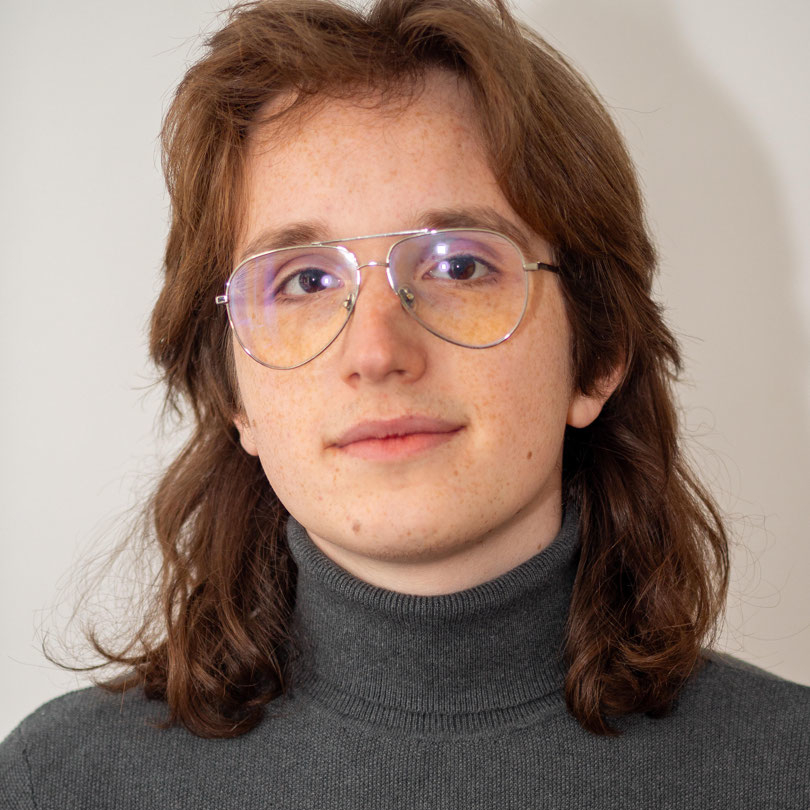
\includegraphics[width=\linewidth]{./src/img/photo_square.jpg}}
    \else
        \fbox{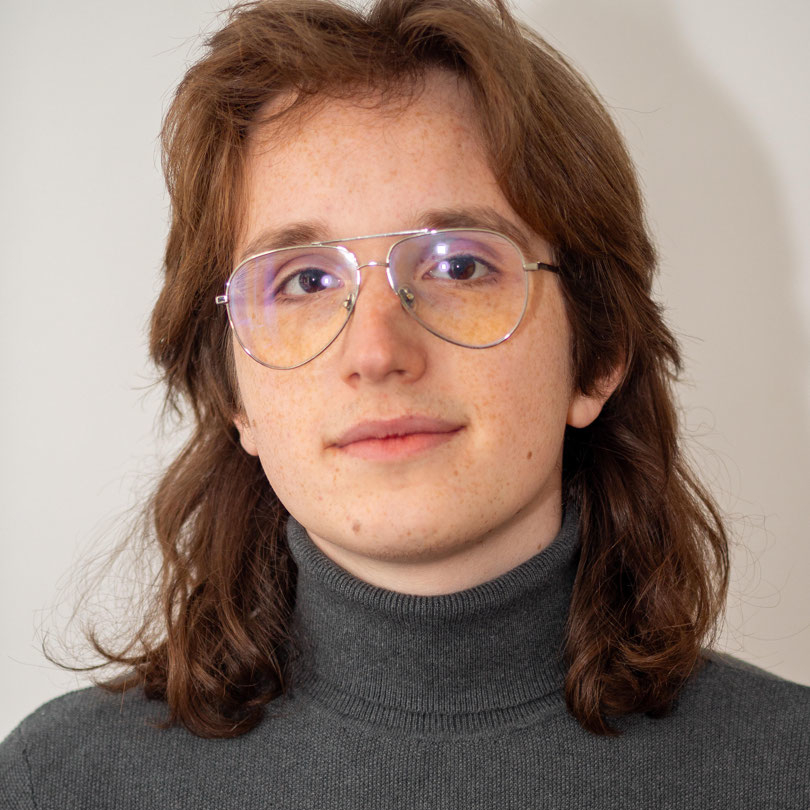
\includegraphics[width=\linewidth,natwidth=810,natheight=810]{./src/img/photo_square.jpg}}
    \fi
\end{minipage}
\hspace{1.5pt} % Adjust this to remove space caused by the fbox
\begin{minipage}[t]{0.49\textwidth} % 45% of the page width for name
    \vspace{-\baselineskip} % Required for vertically aligning minipages
    \colorbox{black}{{\HUGE\textcolor{white}{\textbf{\MakeUppercase{Tymoteusz}}}}} % First name

    \colorbox{black}{{\HUGE\textcolor{white}{\textbf{\MakeUppercase{Burak}}}}} % Last name

    \vspace{6pt}

    \hspace{1.5pt} % Adjust this to align with top text
    {\huge Embedded Systems Engineer} % Career or current job title

\end{minipage}
\begin{minipage}[t]{0.35\textwidth} % 35% of the page width for the first row of icons
    %\vspace{-\baselineskip} % Required for vertically aligning minipages
    \raggedright % Align to left as possible

    % START SUBSTITUTE
    \icon{MapMarker}{8}{\rule{10em}{1em}}\\
    \icon{Phone}{8}{+\rule{2em}{1em} \rule{9em}{1em}}\\
    % END SUBSTITUTE
    \icon{At}{8}{\href{mailto:tymbur@gmail.com}{tymbur@gmail.com}}\\
    \icon{Github}{8}{\href{https://github.com/tym2k1}{github.com/tym2k1}}\\
    \icon{Linkedin}{8}{\href{https://www.linkedin.com/in/tymoteusz-burak/}{linkedin.com/in/tymoteusz-burak}}\\

\end{minipage}
\\ \\

%----------------------------------------------------------------------------------------
% INTRODUCTION, SKILLS AND TECHNOLOGIES
%----------------------------------------------------------------------------------------

% \vspace{-0.6cm} % move the "who am i?" section up
\noindent % Prevents indentation
\begin{minipage}[t]{0.60\textwidth} % 45% of the page width for the introduction text
    \cvsect{Who Am I?}

    \raggedright

    A recent graduate with a passion for innovation, engineering and
    problem-solving. I am eager to pursue a career in research and development (R\&D),
    where I can contribute to fostering innovation and further my
    technical skills.

    Thriving in collaborative environments, I enjoy brainstorming and working in
    a team, where exchanging ideas and leveraging collective strengths leads to
    creative solutions.

\end{minipage}
\hfill % Horizontal space between the minipages
\begin{minipage}[t]{0.35\textwidth}
    \cvsect{Technologies}
    \raggedright % Align to left as possible
    \\
    \colorbox{black}{\textcolor{white}{\raisebox{0.5ex}[10pt][0pt]{\textbf{Linux}}}}
    \colorbox{black}{\textcolor{white}{\raisebox{0.5ex}[10pt][0pt]{\textbf{Shell Scripting}}}}
    \colorbox{black}{\textcolor{white}{\raisebox{0.5ex}[10pt][0pt]{\textbf{Git}}}}
    \colorbox{black}{\textcolor{white}{\raisebox{0.5ex}[10pt][0pt]{\textbf{Yocto}}}}
    \colorbox{black}{\textcolor{white}{\raisebox{0.5ex}[10pt][0pt]{\textbf{Python}}}}
    \colorbox{black}{\textcolor{white}{\raisebox{0.5ex}[10pt][0pt]{\textbf{Docker}}}}
    \colorbox{black}{\textcolor{white}{\raisebox{0.5ex}[10pt][0pt]{\textbf{Nix}}}}
    \colorbox{black}{\textcolor{white}{\raisebox{0.5ex}[10pt][0pt]{\textbf{CI/CD (Github/Gitea Actions)}}}}
    \colorbox{black}{\textcolor{white}{\raisebox{0.5ex}[10pt][0pt]{\textbf{C/C++}}}}
    \colorbox{black}{\textcolor{white}{\raisebox{0.5ex}[10pt][0pt]{\textbf{Buildroot}}}}
    \colorbox{black}{\textcolor{white}{\raisebox{0.5ex}[10pt][0pt]{\textbf{MATLAB}}}}
    \colorbox{black}{\textcolor{white}{\raisebox{0.5ex}[10pt][0pt]{\textbf{LabVIEW}}}}
    \colorbox{black}{\textcolor{white}{\raisebox{0.5ex}[10pt][0pt]{\textbf{LaTeX}}}}
    \\
\end{minipage}

%----------------------------------------------------------------------------------------
% EDUCATION
%----------------------------------------------------------------------------------------

\cvsect{Education}

\begin{entrylist}
    \entry
        {2020 -- 2024}
        {Bachelor's Degree in Automation, Robotics and Control Systems}
        {Gdańsk University of Technology}
        {
        \raggedright
        Thesis:\\
        \textit{Intelligent system for the analysis of a human skeletal model
        in 3D space to support medical diagnosis, rehabilitation and physical
        activity.}
        }
\end{entrylist}

%----------------------------------------------------------------------------------------
% EXPERIENCE
%----------------------------------------------------------------------------------------

\cvsect{Experience}

\begin{entrylist}

    \entry
    {06/2023--Present}
    {Junior Embedded Systems Engineer}
    {3mdeb Sp. z o. o., Gdańsk}
    {
    Working on the Embedded Systems team, I gained hands-on experience across various software engineering areas, including DevOps, code development, and conducting product research. The role also offered opportunities to contribute to collaborative projects while further enhancing my technical expertise.
    \begin{enumerate}
        \raggedright
    \item[$\blacksquare$] Development of custom Linux distributions and firmware for embedded applications using Yocto/Buildroot/OpenWRT, this work was later refined into the \href{https://docs.zarhus.com/}{Zarhus OS, a custom Linux distro.}.
        \begin{enumerate}
            \item[$\blacksquare$] Integrated enhanced security features, such as including Measured Boot, FIDO Device Onboarding, and OTA updates, by leveraging and contributing to existing open-source projects.
            \item[$\blacksquare$] Developed test cases, CI/CD pipelines and documentation.
        \end{enumerate}
        \item[$\blacksquare$] Contributing to the ongoing \href{https://crosscon.eu/}{Cross-platform Open Security Stack for Connected Devices (CROSSCON) Project}:
        \begin{enumerate}
            \item[$\blacksquare$] Co-authored and reviewed validation criteria for the project's technical stack, ensuring compliance with project objectives and industry standards.
            \item[$\blacksquare$] Collaboratively developed high-level architecture for practical use-cases to test real-world applications, contributing to both conceptual design, implementation planning, and prototyping.
            \item[$\blacksquare$] Prepared internal reports on the project's substantive progress, identifying key deliverables and deriving actionable recommendations for the team.
            \item[$\blacksquare$] Authored a blog post: \href{https://crosscon.eu/blog/embracing-ftpm-embedded-arm-devices-insights-and-solutions}{\textit{Embracing fTPM on embedded ARM Devices: Insights and Solutions}}.
        \end{enumerate}
        \item[$\blacksquare$] Public speaking:
        \begin{enumerate}
            \item[$\blacksquare$] \textbf{Yocto Project Developer Day 2024} (Co-Speaker): {\href{https://www.youtube.com/watch?v=W78AKeWh57g}{\textit{Practical Security for Embedded Systems: Implementing TEE and Secure Storage}}}.
            \item[$\blacksquare$] \textbf{Dasharo Developer vPub \#6}: {\href{https://www.youtube.com/watch?v=9vBZeIZnS3o}{\textit{Dasharo Configuration Utility - Status Update}}}.
            \item[$\blacksquare$] \textbf{FOSDEM 2024}: {\href{https://archive.fosdem.org/2024/schedule/event/fosdem-2024-3097-securing-embedded-systems-with-ftpm-implemented-as-trusted-application-in-tee/}{\textit{Securing Embedded Systems with fTPM implemented as Trusted Application in TEE}}}.
            \item[$\blacksquare$] \textbf{Yocto Summit 2023}: {\href{https://www.youtube.com/watch?v=Wg1ZUdwTYNM&t=1s}{\textit{FIDO Device Onboarding: Late-binding Provisioning \& Tales from the Trenches of Bleeding Edge Tech}}}.
        \end{enumerate}
    \end{enumerate}
    }
    \entry
        {05/2021--06/2023}
        {Science Club Member}
        {SimLE Science Club}
        {
            Participated in the Science Club’s \href{https://simle.pl/en/projekty/silverhand/}{"Silverhand"} project, contributing to the second iteration of a prosthetic hand,, and later moved on to the \href{https://simle.pl/en/projekty/simba/}{"SimBa"} sounding rocket project, working within the ground segment team.
        \begin{enumerate}
            \item[$\blacksquare$] Collaborated on bare-metal software for a prosthetic hand using C++ and STM32 microcontroller.
            \item[$\blacksquare$] Worked on designing and implementing the backend for a ground control module of a sounding rocket, using Python, InfluxDB, and Mavlink.
            \item[$\blacksquare$] Prototyped an automated motorized radio antenna and camera mount for rocket tracking, leveraging Python and OpenCV.
        \end{enumerate}
        }

    \entry
        {03/2021--11/2021}
        {Technical Support and Junior Vision Systems Engineer}
        {VisionX, Gdańsk}
        {
        I initially provided general technical support and later transitioned into prototyping industrial vision systems.
        \begin{enumerate}
            \item[$\blacksquare$] Managed a local server running on Windows Server 2019 for remote device access.
            \item[$\blacksquare$] Prototyped/Developed industrial vision systems in LabVIEW / NI Vision:
            \begin{enumerate}
                \item[$\blacksquare$] LED lamp covers burn mark detection.
                \item[$\blacksquare$] Onion rotation detection for food manufacturing.
                \item[$\blacksquare$] Software blueprint for PCB inspections.
            \end{enumerate}
            \item[$\blacksquare$] Collaborated on a QR/Datamatrix reading scanner in C++ and STM32 platform.
        \end{enumerate}
        }
    \end{entrylist}

%----------------------------------------------------------------------------------------
% ADDITIONAL INFORMATION
%----------------------------------------------------------------------------------------

\begin{minipage}[t]{0.5\textwidth}
    \cvsect{Languages}
    \\
    \textbf{Polish}\\Native\\ \\
    \textbf{English}\\Full Professional Proficiency \\
    \textit{ACERT C1 Academic Certificate}
\end{minipage}
\hfill
\begin{minipage}[t]{0.5\textwidth}
    \cvsect{Interests}
    \raggedright % Align to left as possible
    \\
    \colorbox{black}{\textcolor{white}{\raisebox{0.5ex}[10pt][0pt]{\textbf{Music}}}}
    \colorbox{black}{\textcolor{white}{\raisebox{0.5ex}[10pt][0pt]{\textbf{Art}}}}
    \colorbox{black}{\textcolor{white}{\raisebox{0.5ex}[10pt][0pt]{\textbf{FOSS}}}}
    \colorbox{black}{\textcolor{white}{\raisebox{0.5ex}[10pt][0pt]{\textbf{Cybersecurity}}}}
    \colorbox{black}{\textcolor{white}{\raisebox{0.5ex}[10pt][0pt]{\textbf{Control Theory}}}}
    \colorbox{black}{\textcolor{white}{\raisebox{0.5ex}[10pt][0pt]{\textbf{Making}}}}
    \colorbox{black}{\textcolor{white}{\raisebox{0.5ex}[10pt][0pt]{\textbf{Hacking}}}}
    \colorbox{black}{\textcolor{white}{\raisebox{0.5ex}[10pt][0pt]{\textbf{Tinkering}}}}
\end{minipage}

%----------------------------------------------------------------------------------------

% \vfill
% \centering
% \scriptsize
% Wyrażam zgodę na przetwarzanie moich danych osobowych dla potrzeb niezbędnych do realizacji procesu rekrutacji (zgodnie z ustawą z dnia 10 maja 2018 roku o ochronie danych osobowych (Dz. Ustaw z 2018, poz. 1000) oraz zgodnie z Rozporządzeniem Parlamentu Europejskiego i Rady (UE) 2016/679 z dnia 27 kwietnia 2016 r. w sprawie ochrony osób fizycznych w związku z przetwarzaniem danych osobowych i w sprawie swobodnego przepływu takich danych oraz uchylenia dyrektywy 95/46/WE (RODO).

\end{document}
